%%%%%%%%%%%%%%%%%%%%%%%%%%%%%%%%%%%%%%
\section{Estimation with constrains}
%%%%%%%%%%%%%%%%%%%%%%%%%%%%%%%%%%%%%%


%%%%%%%%%%%%%%%%%%%%%%%%%%%%%%%%%
\subsection{General principles}

Occasionally, it might be beneficial to prescribe a specific parametric form for the estimator, denoted as $\hat S = f_{\bf w}(\bf X)$, where ${\bf w}$ represents a vector of parameters. For instance, in scenarios involving two observations, ${\bf X} = [X_1, X_2]^T$, a design constraint might necessitate limiting the search for an estimator to the family of quadratic estimators, characterized by $\hat S = w_0 + w_1 X_1^2 + w_2 X_2^2$. In such situations, the task of designing an estimator consists on identifying the optimal parameter vector ${\bf w}^*$ that minimizes the risk, while adhering to the specified constraints on the estimator structure:
\begin{align}
{\bf w}^* &= \argmin_{\bf w} \EE\{c(S,\hat S)\}
           = \argmin_{\bf w} \EE\{c(S,f_{\bf w}({\bf X}))\} \nonumber\\
          &= \argmin_{\bf w} \int_{\bf x} \int_s c(s,f_{\bf w}({\bf x})) 
                                                 p_{S,{\bf X}}(s,{\bf x}) ds d{\bf x}.
\end{align}

Restricting the estimator to a specific analytic form typically results in a higher risk than what could be achieved with a Bayesian estimator tailored to the same cost function. The exception to this rule occurs when the imposed constraints align with the optimal estimator form, essentially when the Bayesian estimator inherently fits within the specified constraints. Despite potentially incurring higher costs, practical considerations may justify opting for such constrained estimators, such as simplification in design or implementation. An exploration of this concept is presented in Section \ref{sec:est_lineal}, focusing on linear estimators that achieve minimum MSE.

%%%%%%%%%%%%%%%
\begin{example}[{Calculating an Estimator with Constrains}]
\label{CalculoECM_rest}

Continuing the example \ref{CalculoECM2}, we want to calculate the minimum MSE estimator that has the form $\hat{s} = wx^2$. Starting from the conditional risk calculated in \eqref{Est:ECMsx}, the expression of the global average cost can be obtained as
\begin{align}
\label{ec:coste_medio2}
\EE\{c(S,\hat S)\} 
   &= \int_x \EE\{c(S,\hat s)|X=x\} \;p_X(x) dx  \\
   &= \int_x \left(\frac{1}{3}x^2 -\hat{s}x +\hat{s}^2 \right) 
                   p_X(x) dx
\end{align}
Forcing $\hat{s} = wx^2$ and taking into account that $p_X(x)=1$ for $ 0<x<1$ , we get the MSE as a function of $w$.
\begin{align}
\mathbb{E}\{c(S,wX^2)\} 
   & = \int_0^1 \left(\frac{1}{3}x^2 - wx^3 + w^2x^4 \right) dx \\
   & = \frac{1}{9} - \frac{1}{4} w + \frac{1}{5} w^2
\label{Est:ECMwx2}
\end{align}
The value $w^*$ that optimizes \eqref{Est:ECMwx2} can be calculated by differentiation:
\begin{align}
\left. \frac{d}{d\hat{w}} \mathbb{E}\{c(S,w{\bf X}^2)\} \right|_{w=w^*} 
    &= - \frac{1}{4} + \frac{2}{5} w^* =0,
\end{align}
\begin{equation}
\label{eq:sopt_58}
w^* = \frac{5}{8},
\end{equation}
and therefore the estimator is $\hat{s} = \frac{5}{8}x^2$.

\end{example}\vspace{0.4cm}
%%%%%%%%%%%%%


%%%%%%%%%%%%%%%%%%%%%%%%%%%%%%%%%%%%%%%%%%%%%%%%%%%%%%%%%%%%%%%
\subsection{Linear (in the parameters) estimation of minimum MSE}
\label{sec:est_lineal}

In this section we will focus on the study of estimators that are a linear combination of variables related to the observations, using the minimization of the MSE as design criterion. More specifically, we will consider estimators given by the general expression
{\begin{align}
\label{Est:lin_in_w}
\hat S = {\bf w}^\intercal {\bf Z}
\end{align}
where 
\begin{align}
{\bf Z}=\phi({\bf X})
\end{align}
is some known transformation of the observations. The nature of this transformation may depend on the application, but there are some cases of particular interest:
\begin{itemize}
\item \textbf{Linear estimation}: in this case, $\phi$ is the identity function, so that ${\bf Z}={\bf X}$, and the estimator a linear function of the observations
\begin{equation}
\hat S = w_0 X_0 + w_1 X_1 + \dots + w_{N-1} X_{N-1}
\end{equation}
\item \textbf{Linear estimation with independent term}: in this case, ${\bf Z}=(1, {\bf X}^\intercal)^\intercal$ and, thus the estimator includes a constant term $w_0$
\begin{equation}
\label{Est:blin}
\hat S = w_0 + w_1 X_0 + \dots + w_{N} X_{N-1}
\end{equation}
\item \textbf{Polynomial estimation}: in this case, the components of ${\bf Z}$ are monomials of the observational variables. For instance, for a scalar observation $X \in \mathbb{R}$, we can take ${\bf Z} = (1, X, X^2, \ldots X^M)$, for some $M>1$, and the estimation becomes a polynomial of the observation with degree $M$.
\begin{equation}
\hat S = w_0 + w_1 X + w_2 X^2 \dots + w_M X^M
\end{equation}
\end{itemize}}

{Note that in general, the dimensions of ${\bf X}$ and ${\bf Z}$ may be different. Note, also, that, despite the estimator may be a non-linear function of the observation, all estimators given by \eqref{Est:lin_in_w} are linear functions of the parameters. For this reason we will refer to them as estimators that are \textit{linear in the parameters}.}

%where $N$ denotes the number of available observable variables, $\{X_i\}_{i=1}^N$, and $\{w_i\}_{i=0}^{N}$ are the weights that characterize the estimator. In this context, it is common to refer to the term independent of the above expression, $w_0$, as a bias term. For analytic simplicity, it is more convenient to enter the following matrix notation:
%\begin{equation}
%\hat S = w_0 + {\bf w}^T {\bf X} = {\bf w}_{\text{e}}^T {\bf X}_{\text{e}}
%\label{Est:Sestlineal}
%\end{equation}
%where ${\bf w} = [w_1,\dots,w_N]^T$ and ${\bf X} = [X_1,\dots,X_N]^T$ are the (column) vectors  of parameters and observations, respectively, and ${\bf w}_{\text{e}} = [w_0, {\bf w}^T]^T$ and ${\bf X}_{\text{e}} = [1, {\bf X}^T]^T$ are extended versions of these vectors.

By imposing a restriction on the analytic form of the estimator, linear-in-the-parameter estimators will generally obtain lower performance than the optimal Bayesian estimator. However, the interest of linear estimators is justified by their simplicity and ease of design. As we shall see, the linear estimator of minimum MSE depends exclusively on first and second order statistical moments (means and covariances) {associated with the target variable and the transformed observation, ${\bf Z}$}.

%On the other hand, the use of linear estimators is fully justified in certain circumstances, for example when dealing with variables with Gaussian distributions, since, as we saw in the previous section, in this case the Bayesian estimator with the minimum squared mean error has a linear architecture. 


%%%%%%%%%%%%%%%%%%%%%%%%%%%%%%%%%%%%%%%%%%%%%%%%%%%%%%%%%
\subsubsection{Minimization of the {mean squared error}.}% y ecuaciones normales}

We will consider as design criteria the squared error, $c(e) = (s-\hat s)^2$, so the optimal weight vector will be the one that minimizes the MSE risk:
{\begin{equation}
{\bf w}^* 
	= \argmin_{\bf w} \; \EE\{(S - \hat S)^2\} 
    = \argmin_{\bf w}\;  \EE\{(S - {\bf w}^\intercal {\bf Z})^2\}
\end{equation}
and we will refer to the estimator associated with weight vector as $\hat S_\text{LMSE}$: 
$$\hat S_\text{LMSE} = {{\bf w}^*}^T {\bf Z}$$}

{The MSE can be expanded as
\begin{align}
\label{Est:LMSEw}
MSE &= \EE\{(S - \hat S)^2\} = \EE\{(S - {\bf w}^\intercal {\bf Z})^2\}  \nonumber\\
    &= \EE\{S^2\} - 2 \EE\{{\bf w}^\intercal{\bf Z}S\} 
      + \EE\{\left({\bf w}^\intercal {\bf Z}\right)^2\}   \nonumber\\
    &= \EE\{S^2\} - 2 \EE\{S {\bf Z}\}^\intercal {\bf w} 
      + {\bf w}^\intercal \EE\{{\bf Z}{\bf Z}^\intercal\}{\bf w} \nonumber\\
    &= \EE\{S^2\} - 2 {\bf r}_{S{\bf Z}}^\intercal {\bf w} 
      + {\bf w}^\intercal {\bf R}_{\bf Z} {\bf w}
\end{align}
where
\begin{itemize}
\item ${\bf r}_{S{\bf Z}} = \EE\{S {\bf Z}\}$ is the \textbf{cross-correlation vector} between $S$ and ${\bf Z}$
\item ${\bf R}_{\bf Z}=\EE\{{\bf Z}{\bf Z}^\intercal\}$ is the \textbf{autocorrelation matrix} of ${\bf Z}$.
\end{itemize}
Thus, the MSE is a second-degree polynomial in ${\bf w}$}. This is illustrated in Figure \ref{fig:linear_est_error_surface}, which depicts the error surface in a case with two observations. Being the function to minimize quadratic in weights (minimization argument), the error surface will take the form of a $N$ dimensional paraboloid. 
%%%%%%%%%%%%%%
\begin{figure}[htb]
  \begin{center}
  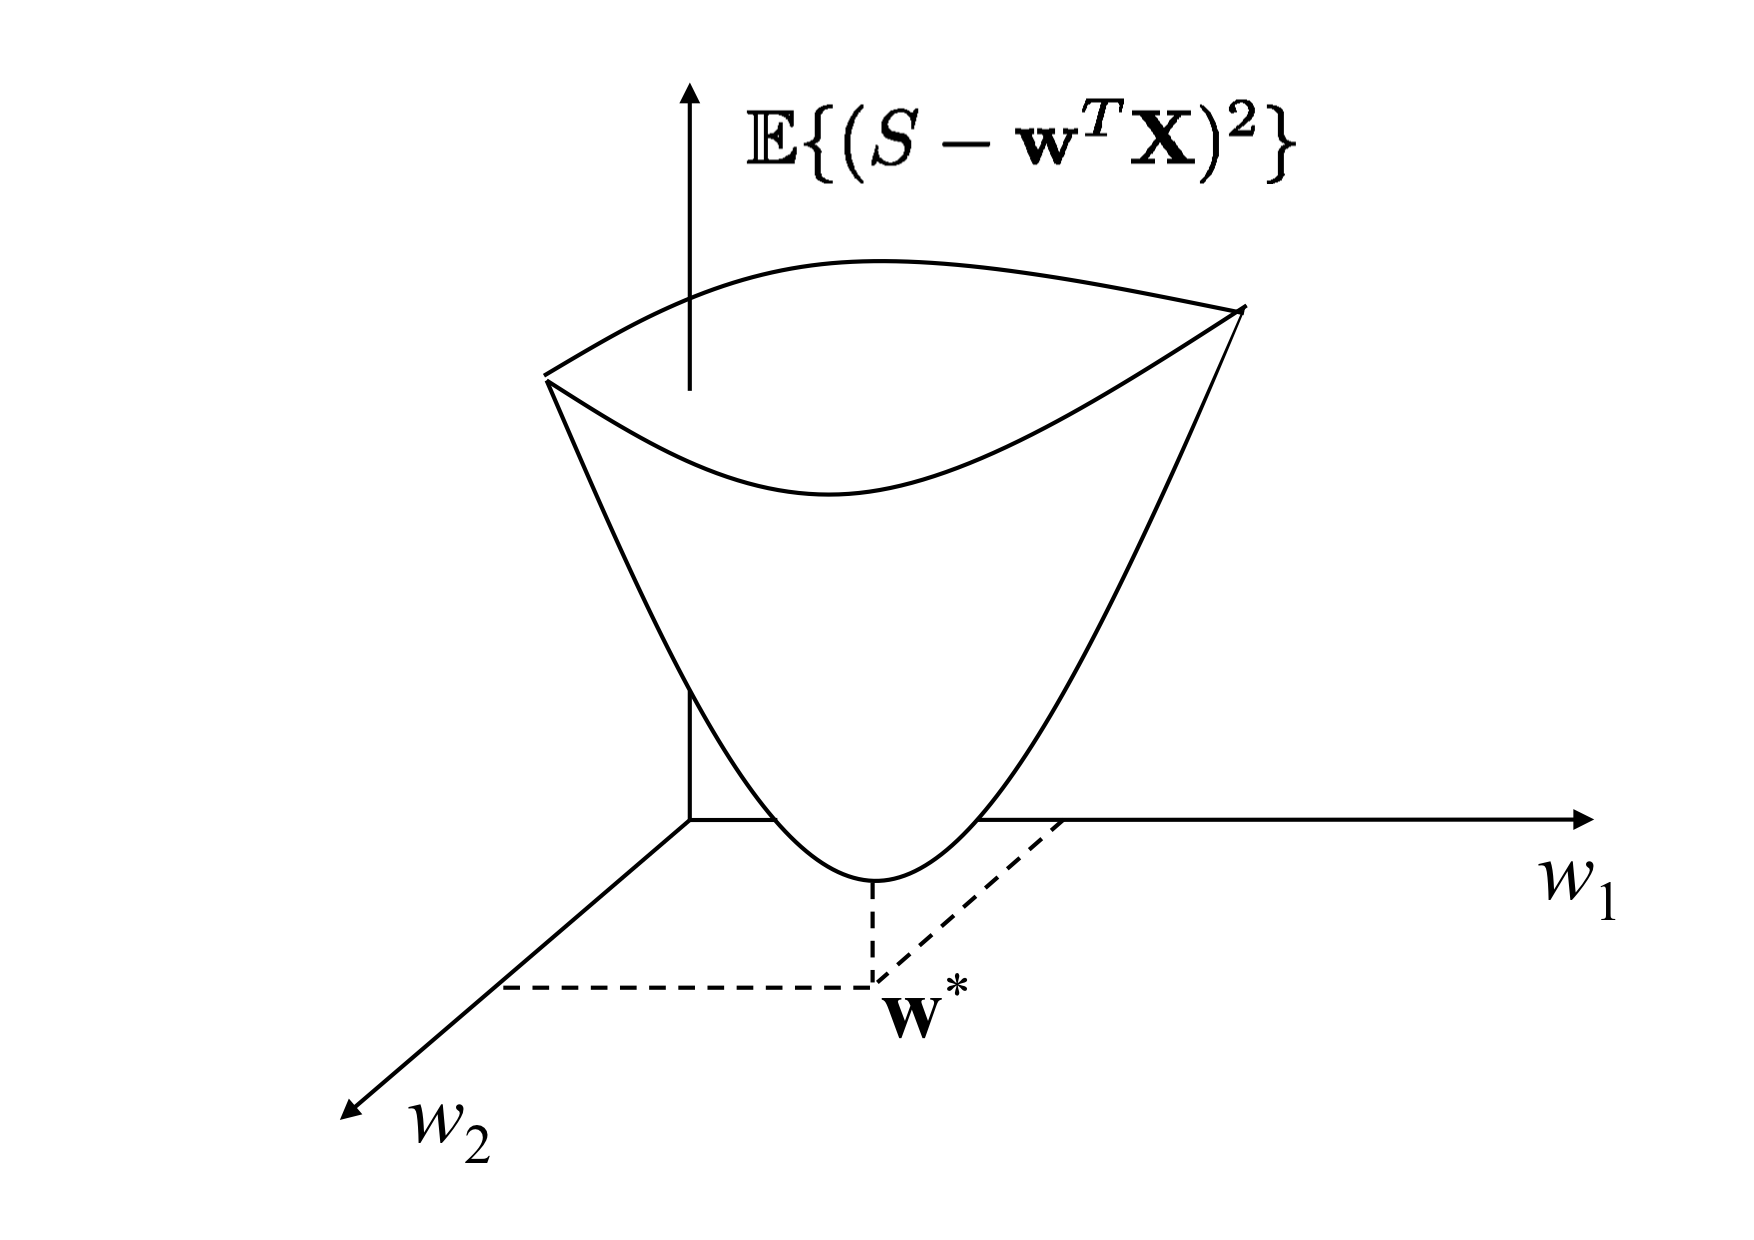
\includegraphics[width=8cm]{Figures//linear_est_error_surface.png}
    \caption{Surface of the MSE for the linear estimator with ${\bf Z}={\bf X}$, as a function of the parameters.}
    \label{fig:linear_est_error_surface}
  \end{center}
\end{figure}
%%%%%%%%%%%%

Since the MSE is non-negative, it is guaranteed to be a convex function of ${\bf w}$ and, thus, its minimum must be located at a point with zero gradient\footnote{The gradient of a function scale $f({\bf w})$ with respect to the vector ${\bf w}$ is defined as a vector formed by the derivatives of the function with respect to each one of the components of $\bf w$: $\nabla_{{\bf w}} f({\bf w}) = \left[\frac{\partial f}{\partial w_1}, \dots \frac{\partial f}{\partial w_N}\right]^T$.} (with respect to ${\bf w}$):
%\begin{align}
%\label{ec:ecs_normales_1}
%\left. \nabla_{\bf w} \EE\{(S - \hat S)^2\} \right|_{{\bf w} = {\bf w}^*} 
% & = \left. -2 \EE\{(S - {\bf w}^T {\bf Z}) {\bf Z}\} \right|_{{\bf w} = {\bf w}^*} = \\
% & = -2 \EE \{(S - {{\bf w}^*}^T {\bf Z}) {\bf Z} \} = {\bf 0}
%\end{align}
{\begin{align}
\label{ec:ecs_normales_1}
\left. \nabla_{\bf w} MSE \right|_{{\bf w} = {\bf w}^*} 
 &= -2 {\bf r}_{S{\bf Z}} + 2 {\bf R}_{\bf Z} {\bf w}^* 
  = {\bf 0}
\end{align}
%The second line of the above expression defines the conditions to be met by the optimal weight vector. Note that this equation is actually a system of $N+1$ equations (as many as dimensions have ${\bf X}_{\text{e}}$) with $N+1$ unknowns (the components of ${\bf w}_{\text{e}^*}$).
%
%In order to find the optimal {weight} vector, it is convenient to rewrite the last line of \eqref{ec:ecs_normales_1} as follows 
%
%\begin{equation}
%\mathbb{E}\{S {\bf X}_{\text{e}} \}
%    = \mathbb{E}\{ {\bf X}_\text{e} ({\bf X}_{\text{e}}^T {\bf w}_{\text{e}}^*)  \}
%\label{Est:EcDelELv}
%\end{equation}
%Defining the cross-correlation vector
%\begin{equation}
%{\bf r}_{S{\bf X}_e} = \mathbb{E}\{S{\bf X}_e\}
%\end{equation}
%and the correlation matrix 
%\begin{equation}
%{{\bf R}_{{\bf X}_e}} = \mathbb{E}\{{\bf X}_e{\bf X}_e^T\}
%\end{equation}
%(which is a symmetric matrix) ec. \eqref{Est:EcDelELv} can be written as
%\begin{equation}
%\label{Est.ec:RxWr}
%{\bf r}_{S{\bf X}_e} = {{\bf R}_{{\bf X}_e}} {\bf w}_{\text{e}}^* 
%\end{equation}
%Thus, the searched weight vector is:
therefore, the optimal weight vector is any solution of
\begin{align}
\label{ec:ecs_normales_2}
{\bf R}_{\bf Z} {\bf w}^* = {\bf r}_{S{\bf Z}}
\end{align}
If the autocorrelation matrix in invertible, we get
\begin{framed}
\begin{equation}
\label{Est.ec:weopt}
 {\bf w}^* = {{\bf R}_{\bf Z}^{-1}} {\bf r}_{S{\bf Z}} 
\end{equation}
\end{framed}}

%
%%%%%%%%%%%%%%%%%%%%%%%%%%%%%%%%%%%%%%%%%%%%%%%%%%%%%%%%
%\subsubsection{Properties of the optimal linear estimator}
%
%Equation \eqref{Est.ec:RxWr} solves the problem of calculating the weights of the estimator $\hat S_\text{LMSE}$. But it is interesting to return to the vector equation  \eqref{ec:ecs_normales_1} to analyze some of its properties. Note that the term in parentheses in this equation is the estimation error
%\begin{equation}
%E^* = S - {{\bf w}_{\text{e}}^*}^T {\bf X}_{\text{e}}
%\end{equation}
%so we can rewrite \eqref{ec:ecs_normales_1} as
%\begin{equation}
%\label{Est:SLMSinsesgado0}
%\mathbb{E}\{E^* {\bf X}_{\text{e}})\} = {\bf 0}
%\end{equation}
%Taking, on the one hand, the first component of this equation (taking into account that $X_{\text{e},1}=1$, and the rest on the other hand, two fundamental properties of the lowest quadratic mean error linear estimator are obtained:
%\begin{description}
%\item[{\bf Property 1:}] The error has zero mean:
%\begin{equation}
%\label{Est:SLMSinsesgado}
%\mathbb{E}\{E^*\} = {\bf 0}
%\end{equation}
%When an estimator has this property it is said that it is {\bf unbiased}.% {Volveremos sobre esta propiedad en la sec. \ref{Est:Sec:CaracterEstim}.}
%\item [{\bf Property 2 (Orthogonality Principle):}] the error is statistically orthogonal to the observations:
%\begin{equation}
%\label{Est:PrincipioOrtV1}
%\mathbb{E}\{E^* {\bf X}\} = {\bf 0}
%\end{equation}
%\end{description}



%%%%%%%%%%%%%%%%%%%%%%%%%%%%%%%%%%%%%%%%%%%%%%%%%%%%%%%%%%%%%%%%%%
\subsubsection{Alternative expression for the linear case}

{We can obtain an alternative expression for the optimal weights in the case of the linear estimator with independent term in \eqref{Est:blin}, which is given by ${\bf Z}=(1, {\bf X}^\intercal)^\intercal$ and can thus be written as
\begin{align}
\hat S = w_0 + {\bf w}_{1:}^\intercal {\bf X}
\end{align}
where ${\bf w}_{1:}$ is the weight vector after removing the first component, $w_0$. To do so, we can re-express \eqref{ec:ecs_normales_2} as the equivalent pair of equations
\begin{equation}
\label{Est:E0}
\EE\{w_0^* + {{\bf w}_{1:}^*}^\intercal {\bf X} \} = \EE\{S\}
\end{equation}
\begin{equation}
\label{Est:Ex}
\EE\{{\bf X}\} w_0^* + \EE\{{\bf X}{\bf X}^\intercal\}{\bf w}_{1:}^* = \EE\{S{\bf X}\}
\end{equation}
that is
\begin{equation}
w_0^* = m_S - {{\bf w}_{1:}^*}^\intercal{\bf m_x}
\end{equation}
\begin{align}
\label{Est:PrincipioOrtV2b}
\EE\{{\bf X} {\bf X}^\intercal \}{\bf w}_{1:}^* = \EE\{S {\bf X}\} - w_0^* {\bf m_X}  
\end{align}
where $m_S=\EE\{S\}$, $m_{\bf X} =\EE\{{\bf X}\}$.} Now using the expressions that relate the correlation and covariance of two variables:
\begin{equation}
\mathbb{E}\{S {\bf X}\} = {\bf v}_{S{\bf X}} + m_S {\bf m_X}
\end{equation}
\begin{equation}
\mathbb{E}\{{\bf X}{\bf X}^\intercal\} = {\bf V_X} + {\bf m_X}{\bf m}_{\bf X}^\intercal
\end{equation}
we get 
{\begin{align}
w_0^* &= m_S  - {{\bf w}_{1:}^*}^\intercal{\bf m_x}  \\
\label{Est:PrincipioOrtV2c}
{\bf v}_{S{\bf X}} + m_S {\bf m_X} 
	&= ({\bf V_X} + {\bf m_X}{\bf m}_{\bf X}^T){\bf w}_{1:}^* + w_0^* {\bf m_X}  
\end{align}}

{Solving these equations for $w_0^*$ and $w_{1:}^*$ we get
%Expanding Ecs. \eqref{Est:SLMSinsesgado} and \eqref{Est:PrincipioOrtV1}, we can obtain the following explicit formulas for the coefficients $w_0^*$ and ${\bf w}^*$ of the estimator:
\begin{framed}
\begin{equation}
w_0^* = m_S - {{\bf w}_{1:}^*}^T{\bf m_x} 
\label{ec:solucionw0}
\end{equation}
\begin{equation}
\label{ec:solucionw}
{\bf w}_{1:}^* = {{\bf V}_{\bf X}^{-1}} \; {\bf v}_{S,{\bf X}}\end{equation}
\end{framed}}

{The optimal estimator is, thus,
\begin{align}
\label{Est:slmse}
\hat{S}_	\text{LMSE} 
	= m_S + {\bf v}_{S{\bf X}}^\intercal {\bf V}_{\bf X} ({\bf X}-{\bf m}_{\bf X})
\end{align}}

The bias term $w_0$ compensates for differences between the means of the target variable and the observations. Therefore, when all the variables involved have zero mean, $w_0^* = 0$, and the estimator is purely linear in the observations.


% In contrast the weight vector ${\bf w}$ minimizes the mean quadratic error of the fluctuations of $S$ around its mean, exploiting for it the existing statistical relation between $S$ and $\bf X$.

%We will dedicate this section to obtain expressions \eqref{ec:solucionw0} and \eqref{ec:solucionw}. The first is a direct consequence of \eqref{Est:SLMSinsesgado} that can be developed as 
%
%\begin{equation}
%m_S - {{\bf w}^*}^T{\bf m_x} - w_0^* =0 
%\end{equation}
%solving for $w_0^*$, we obtain \eqref{ec:solucionw0}.
%
%{We will now search for an expression for ${\bf w}^*$. From \eqref{Est:PrincipioOrtV1} results
%\begin{equation}
%\label{Est:PrincipioOrtV2}
%\mathbb{E}\{(S - {{{\bf w}^*}^T} {\bf X} - w_0^*) {\bf X}\} = {\bf 0}
%\end{equation}
%which can be rewritten as
%\begin{align}
%\label{Est:PrincipioOrtV2b}
%\mathbb{E}\{S {\bf X}\} 
%   &= \mathbb{E}\{({{\bf w}^*}^T {\bf X} + {w_0^*}) {\bf X}\}     \nonumber\\
%   &= \mathbb{E}\{{\bf X} ({{\bf X}^T{\bf w}^*}) \} {+ w_0^*} \mathbb{E}\{{\bf X} \}  \nonumber\\
%   &= \mathbb{E}\{{\bf X} {\bf X}^T \}{\bf w}^* + w_0^* {\bf m_X}  
%\end{align}
%}
%eq. \eqref{Est:PrincipioOrtV2b} becomes 
%\begin{align}
%\label{Est:PrincipioOrtV3}
%{\bf v}_{S,{\bf X}}  
%   &= {\bf V_X}{\bf w}^* + {\bf m_X}{\bf m}_{\bf X}^T{\bf w}^* + w_0^* {\bf m_X} - m_S {\bf m_X}  \nonumber\\ 
%   &= {\bf V_X}{\bf w}^* 
%    + {\bf m_X}(w_0^* + {\bf m}_{\bf X}^T{\bf w}^* - m_S) 
%     \nonumber\\ 
%   &= {\bf V_X}{\bf w}^* 
%\end{align}
%where, in the last equality, we have applied \eqref{ec:solucionw0}. So, solving for ${\bf w}^*$, we get \eqref{ec:solucionw}.



%%%%%%%%%%%%%%%%%%%%%%%%%%%%%%%%%%%%%%%%%%%%%%%%%%%%%%%%%%%%
\subsubsection{Minimum squared mean error}
 
%Here we will calculate the mean squared error associated with the linear estimator of minimum mean squared error, $\hat S_\text{LMSE}$. As commented at the beginning of this section, the mean squared  error obtained will, in general, be higher than the minimum mean squared error of the Bayesian estimator ($\hat S_\text{MMSE}$), except when this last estimator has precisely a linear structure (in this case, it would be the same).

{The minimum MSE can be computed by replacing the optimal weights \eqref{Est.ec:weopt} into
\eqref{Est:LMSEw}
\begin{align}
\label{Est:LMSEw}
MSE^* &= \EE\{S^2\} 
     - 2 {\bf r}_{S{\bf Z}}^\intercal {{\bf R}_{\bf Z}^{-1}} {\bf r}_{S{\bf Z}}  
     + ({{\bf R}_{\bf Z}^{-1}} {\bf r}_{S{\bf Z}} )^\intercal {\bf R}_{\bf Z} 
       {{\bf R}_{\bf Z}^{-1}} {\bf r}_{S{\bf Z}}    \nonumber\\
    &= \EE\{S^2\} 
     - {\bf r}_{S{\bf Z}}^\intercal {{\bf R}_{\bf Z}^{-1}} {\bf r}_{S{\bf Z}}  
\end{align}}

For the linear estimator \eqref{Est:slmse}
%in mean squared error we only have to develop the expression of the MSE, particularizing for $\hat S_\text{LMSE}$ and leaving the result in function of the mathematical expectations of the involved random variables:
%\begin{align}
%\mathbb{E}\{(S - \hat S_\text{LMSE})^2\} 
%   & = \mathbb{E}\{E^*(S - w_0^* - {{\bf w}^*}^T {\bf X})\} \nonumber\\ 
%   & = \mathbb{E}\{E^* S\} 
%     - w_0^* \mathbb{E}\{E^*\} 
%     - {{\bf w}^*}^T \mathbb{E}\{{\bf X}E^*\}  \nonumber\\
%   & = \mathbb{E}\{E^* S\} 
%\end{align}
%where, in the last equality, we have applied the two properties of the minimum quadratic mean error estimator obtained in \eqref{Est:SLMSinsesgado} and \eqref{Est:PrincipioOrtV1}. Operating again the error term, $E^*$, results in
%\begin{align}
%\mathbb{E}\{(S - \hat S_\text{LMSE})^2\} 
%   & = \mathbb{E}\{S (S - w_0^* - {{\bf w}^*}^T {\bf X})\}  \nonumber\\
%   & = \mathbb{E}\{S^2\} 
%     - w_0^* m_S 
%     - {{\bf w}^*}^T ({\bf v}_{S{\bf X}} + m_S {\bf m}_{\bf X})\} \nonumber\\
%   & = \mathbb{E}\{S^2\} - m_S (w_0^* {+} {{\bf w}^*}^T {\bf m}_{\bf X})
%     - {{\bf w}^*}^T {\bf v}_{S{\bf X}}  \nonumber\\
%   & = v_S - {{\bf w}^*}^T {\bf v}_{S{\bf X}} 
%\end{align}
\begin{align}
MSE^* = v_S - {{\bf w}^*}^T {\bf v}_{S{\bf X}} 
\end{align}

%\begin{exercise}[Cálculo del error cuadrático medio para variables con medias nulas]
%Demuestre el resultado \eqref{ec:err_LMSE} para el caso concreto en que $\mathbb{E}\{S\} = 0$ y $\mathbb{E}\{{\bf X}\} = {\bf 0}.$
%\end{exercise}
